As detailed in \refsec{sources of helium}, helium can be produced in tungsten from neutron transmutation and from tritium decay.
This section will focus on comparing these two indirect sources with direct helium implantation in monoblocks.

\subsection{Neutron induced transmutation}

In combination with the Paramak code \sidecite{shimwell_paramak_2021} used for creating the geometry, a neutronics simulation was run to assess the total quantity of helium generation in a monoblock under neutron irradiation with the OpenMC code \sidecite{romano_openmc_2015}, a modern open-source Monte-Carlo neutron and photon transport code.
In this simulation, a neutron source was placed above the monoblock and the total helium production was tallied.
The neutron source corresponds to a \SI{500}{MW} DT source, which gives a neutron generation rate of \SI{1.8}{neutron.s^{-1}} (based on the energy produced by the DT fusion reaction).
50 batches of 1 million neutrons were simulated in order to reduce the stochastic error inherant to Monte-Carlo methods.

The production of helium was found to be more important close to the top surface and to the neutron source (see \reffig{transmutation helium in monoblock}).
It evolves as linearly with the distance from the top surface.
The maximum generation rate is $\approx \SI{7e18}{m^{-3}.s^{-1}}$, which is well below the generation rate from direct implantation.
\reffig{helium generation distribution} was obtained by averaging all the values by distance from the top surface.
The error bars were computed by averaging the standard deviation provided by OpenMC.

\begin{figure*}
    \centering
    \begin{subfigure}{0.5\linewidth}
        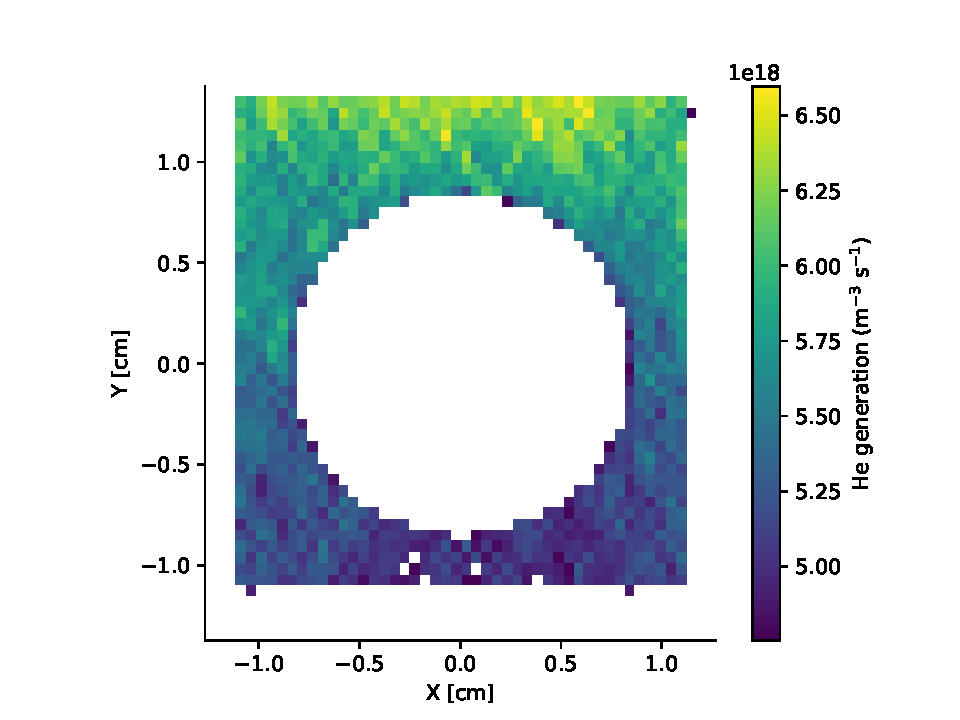
\includegraphics[width=\linewidth]{Figures/Chapter5/helium_transmutation_in_monoblock.pdf}
        \caption{2D distribution}
    \end{subfigure}%
    \begin{subfigure}{0.5\linewidth}
        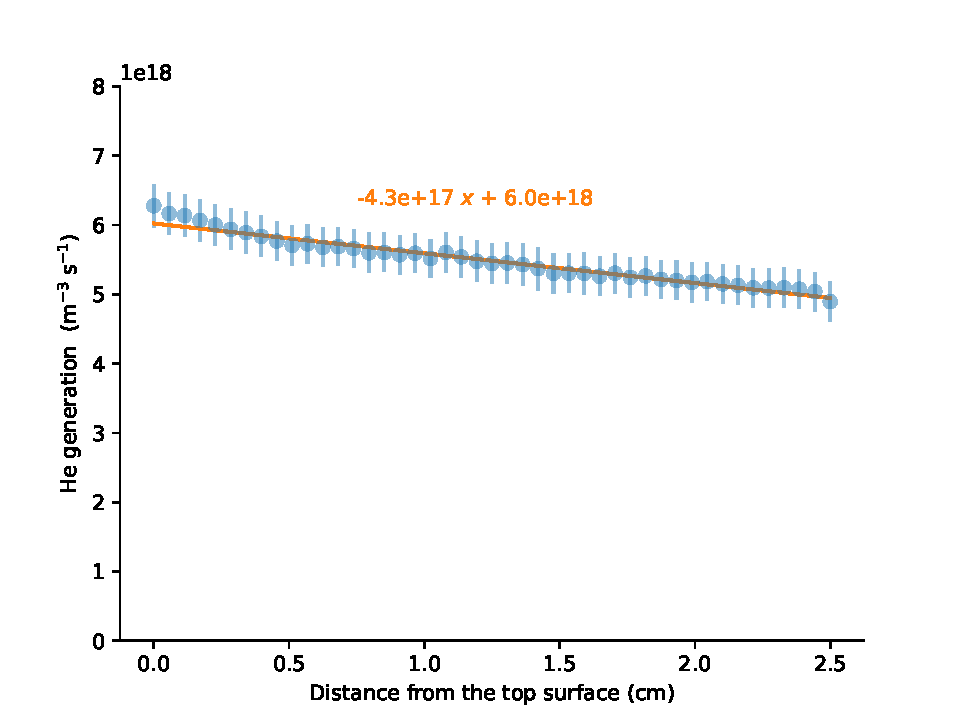
\includegraphics[width=\linewidth]{Figures/Chapter5/he_generation_distribution.pdf}
        \caption{Distribution from the top surface. Errors bars correspond to the 95 \% confidence interval.}
        \labfig{helium generation distribution}
    \end{subfigure}
    \caption{Helium generation via transmutation in a monoblock (only tungsten is shown).}
    \labfig{transmutation helium in monoblock}
\end{figure*}

Note that this is a conservative case as the monoblock simulated is right below the neutron source.
Other monoblocks of the divertor will be tilted and shadowed by others and therefore will interact less with the neutrons.


\subsection{Tritium decay}

\begin{figure}
    \centering
    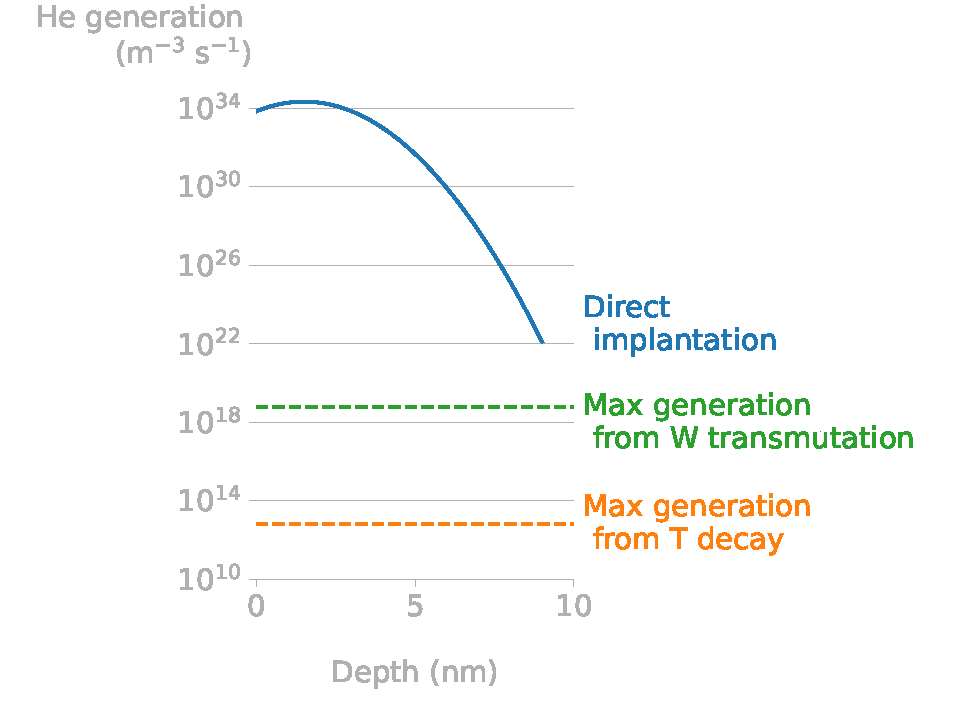
\includegraphics[width=\linewidth]{Figures/Chapter5/helium_generation.pdf}
    \caption{Comparison of the three sources of helium in a monoblock.}
    \labfig{comparison helium generation}
\end{figure}